\documentclass[10pt,letterpaper]{article}
\usepackage[T1]{fontenc}
\usepackage[utf8]{inputenc}
\usepackage{lmodern,microtype}
\usepackage[margin=0.72in,headheight=16pt,footskip=25pt]{geometry}
\usepackage{graphicx,booktabs,tabularx,array,amsmath,enumitem}
\usepackage{xcolor,tikz,tcolorbox,fancyhdr,titlesec,fancyvrb}
\usetikzlibrary{arrows.meta,positioning}
\definecolor{navy}{HTML}{17324D}
\definecolor{teal}{HTML}{237F73}
\definecolor{pale}{HTML}{EFF7F5}
\definecolor{ink}{HTML}{243443}
\definecolor{muted}{HTML}{586877}
\definecolor{amber}{HTML}{A85D1F}
\usepackage[colorlinks=true,linkcolor=teal,urlcolor=teal,
  pdftitle={Functional Recovery from 3D-Print Failures},
  pdfauthor={Failure Detection Project},
  pdfsubject={System architecture, implementation, experimental results and project state}]{hyperref}
\hypersetup{bookmarksnumbered=true}
\urlstyle{tt}
\setlength{\parindent}{0pt}
\setlength{\parskip}{6pt}
\setlength{\emergencystretch}{2em}
\renewcommand{\arraystretch}{1.22}
\setlist[itemize]{leftmargin=1.25em,itemsep=3pt,topsep=3pt}
\setlist[enumerate]{leftmargin=1.45em,itemsep=4pt,topsep=3pt}
\titleformat{\section}{\Large\bfseries\color{navy}}{\thesection}{0.65em}{}
\titleformat{\subsection}{\normalsize\bfseries\color{navy}}{}{0em}{}
\titlespacing*{\section}{0pt}{0pt}{10pt}
\titlespacing*{\subsection}{0pt}{9pt}{3pt}
\pagestyle{fancy}
\fancyhf{}
\fancyhead[L]{\small\color{muted}FUNCTIONAL RECOVERY FROM 3D-PRINT FAILURES}
\fancyhead[R]{\small\color{muted}Project report}
\fancyfoot[L]{\small\color{muted}Research prototype\quad\textbullet\quad 3 November 2026}
\fancyfoot[R]{\small\color{muted}\thepage}
\renewcommand{\headrulewidth}{0.3pt}
\newcolumntype{Y}{>{\raggedright\arraybackslash}X}
\newcommand{\code}[1]{\texttt{\detokenize{#1}}}
\newcommand{\repourl}{https://github.com/3D-Printing-Failure-Detection/failure-detection/blob/work/neural-local-recovery}
\newcommand{\repo}[2]{\href{\repourl/#1}{#2}}
\newcommand{\note}[1]{\begin{tcolorbox}[colback=pale,colframe=teal!55,boxrule=0.5pt,arc=2pt,left=8pt,right=8pt,top=5pt,bottom=5pt]#1\end{tcolorbox}}
\newcommand{\nextpage}{\clearpage}
\DefineVerbatimEnvironment{Code}{Verbatim}{fontsize=\small,frame=single,rulecolor=\color{teal!40},framesep=6pt}
\begin{document}
\color{ink}

{\color{teal}\bfseries SYSTEM OVERVIEW AND CURRENT STATE}\par
\vspace{8pt}
{\fontsize{29}{33}\selectfont\bfseries\color{navy}Functional recovery\newline from 3D-print failures}\par
\vspace{5pt}
{\large How the loop works, what changed, and what the evidence supports}\par
\vspace{9pt}

\note{\textbf{The goal: finish a part that still does its job after a printing error.}
A deformed cup that still holds liquid can be a success. A visually similar cup
that leaks is a failure. The controller should intervene only when doing so helps
preserve the part's functional requirements.}

The project is a Python research prototype that measures each printed layer,
estimates how commands turn into deposited material, and chooses whether to
continue, replace the remaining layer plan, or stop. The established \code{contour}
policy separates inner and outer boundaries when predicting deformation. Trained
models and a free local Qwen supervisor are implemented. The latest complete
policy increases completions but also defective finishes. Some earlier successes
remain lost. An earlier candidate failed its fresh test. The overall objective
is still unmet; historical regression and a new frozen test are required.

\begin{center}
\begin{tabular*}{\linewidth}{@{\extracolsep{\fill}}lll@{}}
\toprule
{\Large\bfseries\color{teal}141/240} & {\Large\bfseries 136/240} & {\Large\bfseries 133/240}\\
Joint camera + Qwen & Prior neural + Qwen & Matched analytical\\
\bottomrule
\end{tabular*}
\end{center}
These are functional completions on the same \emph{240 simulated fault cases
across all four parts}. Defective finishes are respectively \textbf{five, one
and one}; all pass 48 clean controls. The latest policy preserves every active
recovery baseline's success but still loses five ignore successes. Qwen makes
527 actual requests and matches neural-only. These are consumed development
cases. The higher completion count does not waive the defect regression.

\subsection*{Where the project stands}
\begin{tabularx}{\linewidth}{@{}p{1.45in}Y@{}}
\toprule
Implementation & Working simulation/evaluation pipeline; latest predictor is opt-in.\\
Validation & The complete first fresh comparison fails acceptance: neural + Qwen 126/240, contour 128/240, preventive analytical recovery 133/240. All 4,320 runs are audited.\\
Latest checks & The 5,760-row comparison finds 141/240 completions but five defects, versus matched analytical 133/240 and one defect. A correction guard passes its 42-row gate; the full rerun is running. Fresh-test superiority is unproven.\\
Hardware & Bambu integration code exists, but physical recovery is unvalidated. The live entry point still constructs the original rule policy.\\
Integration & \href{https://github.com/3D-Printing-Failure-Detection/failure-detection/pull/1}{PR \#1} merged into main. Neural work is on \code{work/neural-local-recovery}, in draft \href{https://github.com/3D-Printing-Failure-Detection/failure-detection/pull/2}{PR \#2}.\\
\bottomrule
\end{tabularx}

\subsection*{What this report covers}
The system and its functional contract (page 2); observation and prediction
(page 3); recovery decisions and cost assumptions (page 4); implementation
history and evaluation design (page 5); results (page 6); limitations and next
work (page 7); code and operation (page 8); evidence and reproducibility (page 9);
trained recovery and local supervision (from page 10).

{\small\color{muted}Historical contour snapshot: \code{9770276}. Neural experiments
retain separate frozen source hashes. Results describe simulated experiments,
not real-printer reliability. Detailed evidence is linked
throughout the report.}

\nextpage
\section{The system and its functional contract}

A part is represented as a stack of planar material regions, each with a height.
The region can contain holes and multiple components. Geometry comes from YAML
constructive shapes, STL cross-sections, or parsed sliced G-code. A separate
functional specification expresses what the finished part must retain.

\begin{center}
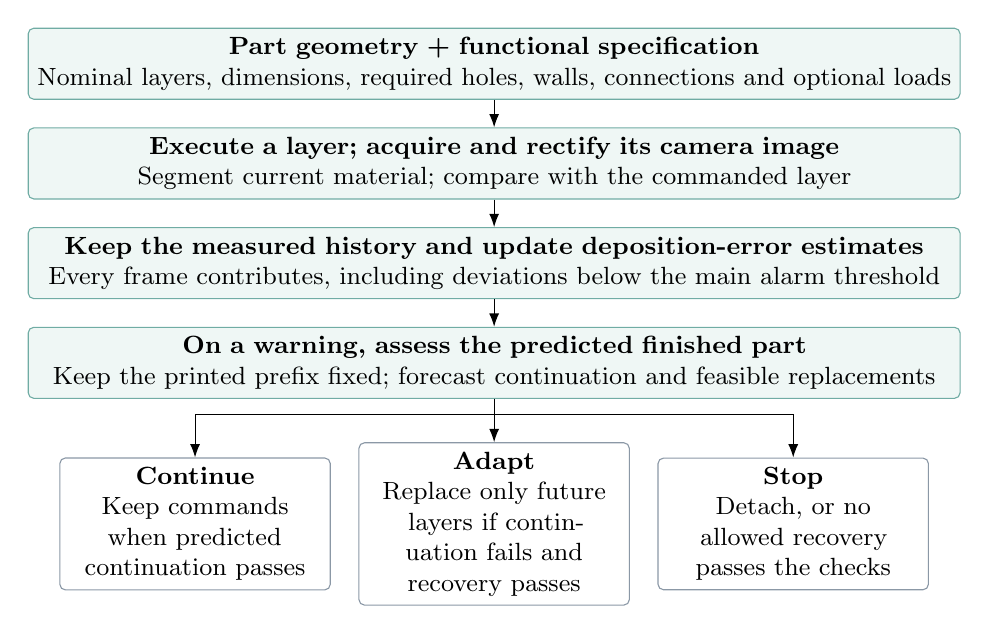
\begin{tikzpicture}[>=Latex,
 stage/.style={draw=teal!65,fill=pale,rounded corners=2pt,text width=11.6cm,align=center,minimum height=0.85cm,font=\small},
 action/.style={draw=navy!50,fill=white,rounded corners=2pt,text width=3.2cm,align=center,minimum height=1.1cm,font=\small}]
\node[stage] (input) {\textbf{Part geometry + functional specification}\\Nominal layers, dimensions, required holes, walls, connections and optional loads};
\node[stage,below=0.35cm of input] (measure) {\textbf{Execute a layer; acquire and rectify its camera image}\\Segment current material; compare with the commanded layer};
\node[stage,below=0.35cm of measure] (state) {\textbf{Keep the measured history and update deposition-error estimates}\\Every frame contributes, including deviations below the main alarm threshold};
\node[stage,below=0.35cm of state] (assess) {\textbf{On a warning, assess the predicted finished part}\\Keep the printed prefix fixed; forecast continuation and feasible replacements};
\node[action,below=0.55cm of assess] (adapt) {\textbf{Adapt}\\Replace only future layers if continuation fails and recovery passes};
\node[action,left=0.35cm of adapt] (cont) {\textbf{Continue}\\Keep commands when predicted continuation passes};
\node[action,right=0.35cm of adapt] (stop) {\textbf{Stop}\\Detach, or no allowed recovery passes the checks};
\draw[->] (input)--(measure);
\draw[->] (measure)--(state);
\draw[->] (state)--(assess);
\draw[->] (assess)--(adapt);
\draw[->] (assess.south) -- ++(0,-0.2) -| (cont.north);
\draw[->] (assess.south) -- ++(0,-0.2) -| (stop.north);
\end{tikzpicture}
\end{center}
{\small\color{muted}Continue and adapt return to the next layer. The diagram
summarizes the experimental guarded/contour path; a detach alarm stops directly.}

\subsection*{What is checked}
\begin{tabularx}{\linewidth}{@{}p{1.5in}Y@{}}
\toprule
Container function & Solid base, closed walls and an allowed capacity range. Closure is inferred from cross-sectional geometry, not a physical leak test.\\
Dimensions and fit & Through-hole diameter and center tolerance, including the intersection of holes through the stack.\\
Material and structure & Minimum wall thickness, allowed material volume, required components and feature area.\\
Layer support & Excess overhang relative to the nominal design; optional finite-element checks can filter load-bearing candidates.\\
\bottomrule
\end{tabularx}

\subsection*{Success is an observed outcome, not an action name}
In simulation, a successful completion means the full deposited stack passes the
original specification. An adaptation is only an attempted recovery. A stop
remains a failed in-place completion even if a later clean restart is assumed in
a cost calculation. In a live print, geometry is estimated from images, so a
passing software verdict is not independently verified physical success.

\nextpage
\section{Seeing and predicting the build}

\subsection*{Perception used in the reported experiments}
The established contour benchmark uses classical OpenCV perception. New trained
models are described on page 10. A calibrated camera view is rectified to the current layer plane. The
segmenter extracts material contours from controlled current-layer illumination.
The detector measures boundary deviation and uses geometric changes to assign a
failure label. Its main deviation threshold is 1 mm.

The experimental policies also issue functional warnings for smaller changes:
a thinning wall, a blocked or displaced required hole, an opening in a container,
lost material, a broken connection or deteriorating support. Measurements are
retained even when the detector says the frame is normal.

\subsection*{Three distinct geometries}
\begin{tabularx}{\linewidth}{@{}p{1.55in}Y@{}}
\toprule
Nominal design & The original intended geometry, used as a reference for function and support.\\
Commanded geometry & The layer the printer is asked to produce; compensation can make this differ from the desired deposited shape.\\
Measured / predicted deposit & What the camera observes now, and what the estimator expects the current or replacement commands to produce later.\\
\bottomrule
\end{tabularx}
For example, if commands consistently deposit material 1 mm to the right, a
desired wall at its nominal position may require a command displaced to the
left. Simply asking for the desired final outline would leave the bias in place.

\subsection*{The contour predictor}
\begin{enumerate}
\item Estimate global translation between commanded and measured outlines.
\item Associate exterior rings with exterior rings and hole rings with holes.
Use one-to-one associations based on geometry after translation; compute nearest
positions along continuous measured contours.
\item Fit local offsets, smoothed at a 1 mm spatial scale. Keep exterior and
interior samples separate when forecasting and computing compensation.
\item Retain four recent residual fields. Estimate a median change between
fields, clip each coordinate of the trend to $\pm0.5$ mm per layer, extrapolate
for at most three layers, then hold that estimate for the more distant future.
\end{enumerate}

The previous fit could match an outside wall point to the inside of the same
wall when the deformation approached the wall thickness. This could create a
false opening in the forecast. Separating boundary roles directly addresses that
failure mode. If the observed ring counts are incompatible, the affected role
falls back to the earlier residual fit; the measured shape is not repaired.

\subsection*{Forecasting and inverse compensation}
Writing a geometric warp as $T_u$, the forward model is
\[
\widehat{\text{deposit}}_{k+h}=T_{u_{k,h}}(\text{command}_{k+h}).
\]
The inverse step uses four fixed-point updates to find commands whose predicted
deposit approaches each recovery target. Candidate checks then evaluate the
measured prefix plus this forecast, not the command shapes alone.

\note{\textbf{This is an analytical short-history estimator.} Its uncertainty
scale comes from spatial resolution and changes between observations. It is not
a calibrated probability of failure, and simulator truth is never passed to it.}

\nextpage
\section{How the controller chooses recovery}

\subsection*{Function first; intervene only when continuation fails}
The \code{contour} policy inherits the guarded decision process. A passing
continuation is retained without requesting a replan just to improve geometric
margin. A warning is still assessed; it is not suppressed because an earlier
frame already warned. The controller supplies the remaining adaptation budget
and a replacement-plan validator as explicit decision inputs.

\begin{enumerate}
\item \textbf{Validate and forecast continuation.} If the measured prefix plus
predicted remaining deposit passes the function checks, continue.
\item \textbf{Generate recovery targets if allowed.} Try a held measured shape,
a bounded return or partial correction, and slower blends. Permanent deformation
is allowed when it still meets the specification.
\item \textbf{Convert targets into compensating commands.} Reject replacements
that change the remaining layer count/heights or violate the backend validator.
MuJoCo checks bed, build-height and inspection-field bounds.
\item \textbf{Check function and select.} Among passing, executable candidates,
rank by uncertainty-envelope margin, central margin, smaller command change,
then nominal fidelity. Optional FEA operates on predicted deposits.
\item \textbf{Stop if none passes.} An exhausted budget cannot force a passing
continuation to stop, but it rules out another adaptation when continuation fails.
\end{enumerate}

The default cap is three adaptations per print. Printed layers remain fixed in
all candidate checks. Forecasting a healthy future cannot erase a measured
broken base or a previously opened wall.

\subsection*{A correction budget inspired by the Colab notebook}
The notebook separated functional adequacy, correction reachability and expected
cost. We adapted those ideas into the existing geometry loop:
\[
N_{\mathrm{required}}=\left\lceil
\frac{\text{estimated correction (mm)}}{\text{assumed correction per layer (mm)}}
\right\rceil.
\]
The default assumption is 0.25 mm of correction per layer. A 2 mm displacement
therefore needs at least eight layers under this model. The budget describes a
sampled fitted displacement schedule, not a measured physical printer limit.
When full restoration will not fit, held or partial shapes can still be accepted
if their predicted function passes.

\subsection*{Cost is logged without inventing success probabilities}
The notebook's recovery-versus-restart comparison was extended to include
continuing. In one common cost unit, let $C_c$ be remaining continuation cost,
$C_a$ recovery cost, $C_i$ intervention cost and $C_r$ a full restart cost:
\begin{align*}
E[C_{\mathrm{continue}}]&=C_c+(1-p_c)C_r,\\
E[C_{\mathrm{recover}}]&=C_i+C_a+(1-p_a)C_r.
\end{align*}
Recovery is cheaper when
\[
p_a-p_c>\frac{C_i+C_a-C_c}{C_r}.
\]
The current policy logs the required success gain using a material-volume proxy.
Unknown probabilities stay unknown; expected savings remain null. This is a
diagnostic calculation, not the implemented intervention gate or a measured
time-saving claim. The implemented gate is predicted functional feasibility.

\nextpage
\section{What changed and how it was evaluated}

\subsection*{The implementation progression}
\begin{tabularx}{\linewidth}{@{}p{1.05in}Y@{}}
\toprule
\code{ours} & Original function-checking rule policy; remains the default.\\
\code{measured} & Retains measured state on every layer and adds functional warnings.\\
\code{predictive} & Adds persistent command-to-deposit error prediction and inverse compensation.\\
\code{functional} & Ranks feasible plans by functional margin. Experiments exposed unnecessary replans and interaction with the action cap.\\
\code{guarded} & Keeps passing continuation, checks action budget and bounds before selection, and uses correction budgets and smaller-change tie-breaking.\\
\code{contour} & Keeps guarded decisions and replaces the residual estimator with separate exterior/hole contour fitting.\\
\bottomrule
\end{tabularx}
The benchmark also provides ignore, scrap-on-alarm and alert-only baselines.
Earlier work added the multi-rig backend, continuous monitoring, regression
coverage and corrections to geometry parsing, rasterization, G-code handling,
FEA filtering and live-interface checks. A later cache fix replaced recycled
object IDs with persistent tokens and included the full nominal reference.

\subsection*{What MuJoCo supplies}
Position-actuated stages execute extrusion waypoints; realized nozzle motion
relative to the bed is converted into geometric beads. Small bead-fusion closing
is applied before the prescribed failure, then a perspective RGB image is
rendered and rectified. The policy sees this image-derived measurement.

\begin{tabularx}{\linewidth}{@{}lYYY@{}}
\toprule
Profile & Motion & Bed (mm) & Line width (mm)\\
\midrule
Cartesian & Independent head axes & $220\times220$ & 0.42\\
CoreXY & Ideal diagonal motor coordinates & $256\times256$ & 0.45\\
Moving bed & X/Z head; moving Y bed & $180\times180$ & 0.48\\
\bottomrule
\end{tabularx}
Camera view, color and noise also vary. These are illustrative rigs, not calibrated
commercial-printer models. The simulator does not model molten plastic, adhesion,
thermal contraction or a complete firmware interpreter.

\subsection*{Latest frozen experiment}
Four parts (bracket, cup, mug, spacer) face five prescribed failures: collapse,
warp, shift, under-extrusion and detach, plus clean controls. The latest comparison
uses \code{ignore}, \code{ours}, \code{guarded} and \code{contour}.

\begin{tabularx}{\linewidth}{@{}YYYr@{}}
\toprule
Study & Profiles & Seeds & Runs\\
\midrule
Main & All three & 10 & 288\\
Fresh-seed check & Cartesian & 22 and 23 & 192\\
Selected rescue confirmation & Cartesian cup starvation & 0 & 4\\
\bottomrule
\end{tabularx}
The first two studies contain 100 paired failure scenarios and 20 paired clean
scenarios across four methods. The selected rescue is excluded from benchmark
totals. Every monitored print begins at layer zero; faults are not cleared by
adaptation. Parameters were frozen before the fresh seeds. The same fault draws
repeat across profiles, so scenario counts are not independent failure samples.

\nextpage
\section{Measured results}

\begin{tabularx}{\linewidth}{@{}Yrrrrr@{}}
\toprule
Policy & Main & Fresh & Total good & Scrap & Defective\\
 & /60 & /40 & /100 & /100 & /100\\
\midrule
Ignore & 33 & 20 & 53 & 0 & 47\\
Original rules & 24 & 14 & 38 & 55 & 7\\
Guarded & 29 & 14 & 43 & 57 & 0\\
\textbf{Contour} & \textbf{40} & \textbf{22} & \textbf{62} & \textbf{37} & \textbf{1}\\
\bottomrule
\end{tabularx}

\begin{center}
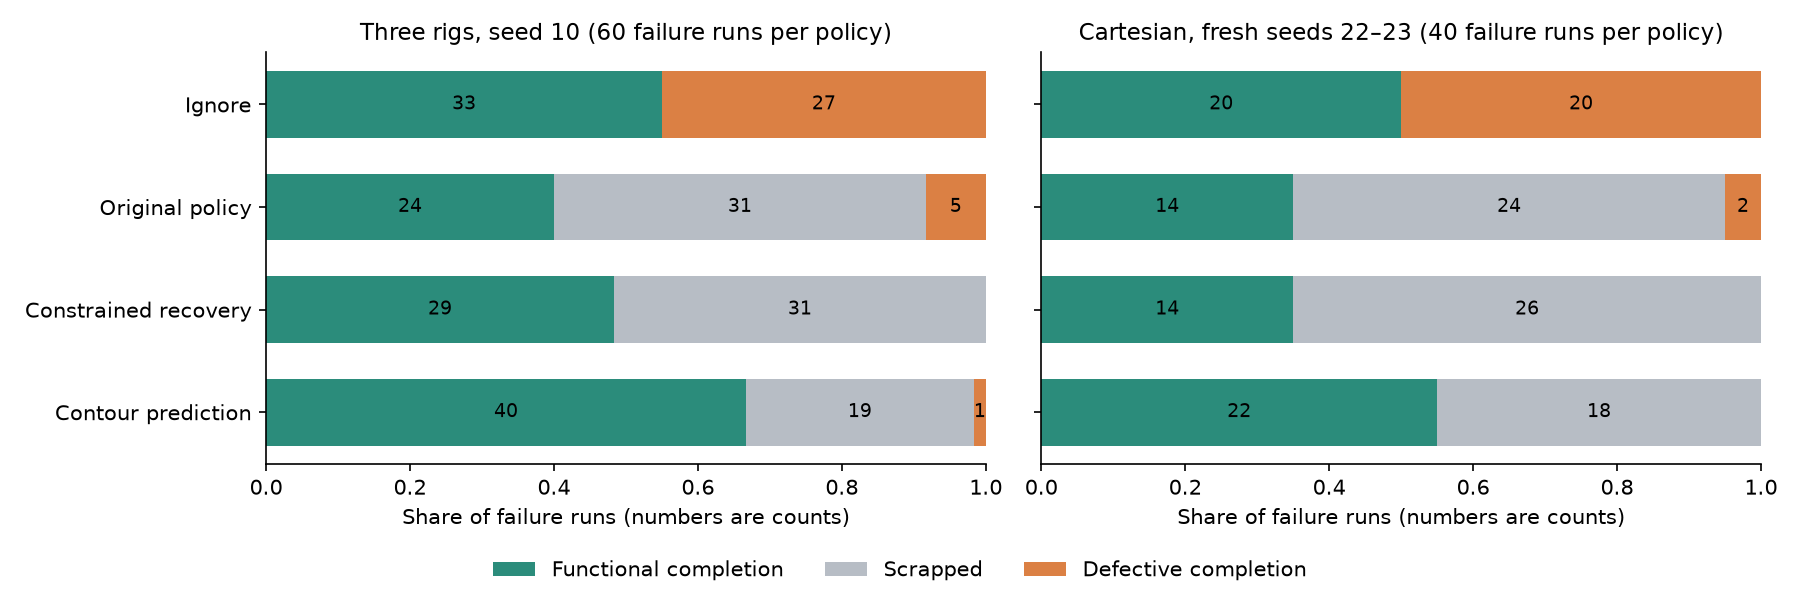
\includegraphics[width=\linewidth]{docs/validation/contour/outcomes.png}
\end{center}
{\small\color{muted}Counts are from the final audited runs. Scraps and defective
finishes are displayed separately from functional completion.}

\subsection*{What improved}
\begin{itemize}
\item \textbf{Versus guarded:} twenty gained successes and one lost rescue,
for a net gain of nineteen. All twelve main-study warped/collapsed cup and mug
cases that guarded lost are restored; eight more are restored on fresh seeds.
\item \textbf{Versus ignoring failure:} all 53 successful prints are preserved,
and nine additional prints are genuinely rescued. Thus 62/100 is not a 62\%
rescue rate among harmful failures: the rescue count is 9 of 47 ignore failures.
\item \textbf{Fresh-seed consistency:} seed 22 improves from 6/20 guarded successes
to 10/20; seed 23 improves from 8/20 to 12/20. No guarded success is lost there.
\end{itemize}

\subsection*{Did the forecast itself improve?}
Eight selected, untouched development trajectories supplied identical commands
and camera measurements to both estimators. On the five functional trajectories,
false full-continuation failure forecasts fell from \textbf{19/70 sampled
checkpoints to 0/70}. On the three defective trajectories, missed failure
forecasts increased from \textbf{10/42 to 11/42}. These are correlated development
checkpoints, not calibrated probabilities or an independent classifier test.

One-step forecasts were scored before the current measurement entered the model.
For the cup-collapse trajectory, mean boundary error fell from 1.116 mm to
0.313 mm. Better contour accuracy helps, but it does not guarantee a correct
functional verdict in every case.

\note{\textbf{Original contour validation:} 53 tests passed; one optional module skipped.
All 80 clean runs passed with zero alarms in 6,000 monitored frames. All 216
overlapping baseline replays matched the prior study. The audit covers all 484
final runs with stable source hashes and complete, unique scenario grids.}

\nextpage
\section{Readiness, limitations and next work}

\subsection*{Two observed problems remain visible}
\textbf{Lost moving-bed mug rescue.} At seed 10, guarded rescues a shifted mug
with adaptations at layers 108 and 113. Contour adapts at 108 and stops at 111;
every candidate reports one leaking layer. The logs establish the estimator's
belief, not whether the stopped physical geometry was actually open. This is
counted as a lost guarded success.

\textbf{Missed spacer tolerance.} A seed-10 Cartesian spacer finishes after two
adaptations, but its actual through-hole is 8.4 mm against an 8.5 mm minimum.
Guarded stops this case. The new policy's measured-prefix check passes with only
0.013 normalized margin. Its uncertainty envelope perturbs future layers, not
the already-measured prefix; at completion no future layers remain. This is
counted as a defective finish, with the original threshold unchanged.

\subsection*{Implemented is not the same as validated}
\begin{tabularx}{\linewidth}{@{}p{1.35in}Y@{}}
\toprule
Simulation recovery & Runs end to end with classical perception; strongest current evidence is the paired geometric benchmark.\\
Live Bambu path & Camera calibration, telemetry, pause/cancel and replacement-job code exist. Physical resume behavior and recovery remain unvalidated. \code{run_live} still selects \code{RulePolicy}; contour is not wired into live mode.\\
Optional FEA & Coarse linear-elastic screening exists, including loads and leak/connectivity checks. Latest success counts are geometry-only, not load-bearing validation.\\
Neural / LLM paths & A temporal network, optional learned camera and actual local Qwen supervision now run in separate experiments. They were not used to produce the historical contour results on page 6; see pages 10--11.\\
Deployment & Open PR; experimental policies are opt-in. Existing hardware/platform/parser concerns require their own checks before release.\\
\bottomrule
\end{tabularx}

\subsection*{Prioritized next work}
\begin{enumerate}
\item \textbf{Model measurement uncertainty on the printed prefix.} Evaluate
confidence for hole size, wall thickness and openings near tolerance boundaries,
using labeled geometry or independent physical measurements.
\item \textbf{Resolve the moving-bed shift regression.} Compare command choices,
observed contours and actual deposits through the first adaptation. Preserve
this case as a regression when changing compensation or estimator selection.
\item \textbf{Expand validation.} Add fault seeds, shapes, lighting/calibration
variation and eventually real camera data. Keep false interventions, genuine
rescues and defective completions separate; reserve new data before tuning.
\item \textbf{Integrate and qualify hardware deliberately.} Add policy selection
to the live path, exercise it without commanding recovery first, then validate
position retention, clearance and resume behavior before physical recovery trials.
\end{enumerate}

The useful current conclusion is that separating wall contours substantially
improves functional completion in the tested conditions. It does not establish
unattended real-printer reliability or justify treating margins as success
probabilities. The new policy remains opt-in.

\nextpage
\section{Code map and operation}

\begin{tabularx}{\linewidth}{@{}p{2.7in}Y@{}}
\toprule
Repository area & Responsibility\\
\midrule
\code{parts/*.yaml}; \code{recovery/parts.py} & Example parts, geometry loading and functional specs.\\
\code{recovery/models/classical.py} & Image segmentation and geometric failure detection.\\
\code{recovery/loop/controller.py} & Per-layer observation, warnings, decisions and printer actions.\\
\code{recovery/loop/contour.py} & New residual estimator, forecast and inverse compensation.\\
\code{recovery/loop/guarded.py} & Continuation-first policy, candidate filtering and selection.\\
\code{recovery/loop/recoverability.py} & Correction-layer budget and expected-cost diagnostics.\\
\code{recovery/geometry/}; \code{recovery/fea/} & Contour operations, targets, function checks and optional structural screening.\\
\code{recovery/printer/}; \code{recovery/live.py} & MuJoCo/Bambu backends and live entry point.\\
\code{recovery/eval/mujoco_eval.py} & Paired scenarios, final truth-based evaluation and manifests.\\
\code{tools/}; \code{docs/validation/} & Auditing, plotting, diagnostics and committed compact evidence.\\
\bottomrule
\end{tabularx}

\subsection*{Run the current simulation comparison}
Use the existing environment on this machine. Long evaluations should start
inside tmux; keep raw outputs on the data volume and choose a fresh output
directory for every run.
\begin{Code}
tmux new -A -s failure-recovery
cd /home/ishaan/failure-detection
export OPENBLAS_NUM_THREADS=1 OMP_NUM_THREADS=1 MUJOCO_GL=egl
FD_RESULTS=/mnt/data/ishaan/hri-workspace/failure-detection

.venv/bin/python -m recovery.cli mujoco-eval \
  --methods ignore ours guarded contour \
  --n 1 --seed 10 --workers 8 \
  --out "$FD_RESULTS/new-main-study"
\end{Code}
The fresh-seed study adds \code{--profiles cartesian --n 2 --seed 22} and a
different output directory. Exact audit/plot commands are in
\repo{docs/contour-prediction-trial.md}{the contour prediction trial report}.
For environment setup elsewhere, use \code{requirements-sim.txt} and a suitable
data disk. The local \code{.venv} is a symlink into that disk.

\subsection*{Tests, demos and persistent sessions}
\begin{Code}
.venv/bin/python -m pytest -q
tmux attach -t failure-recovery
\end{Code}
Detach from tmux with Ctrl-b, then d. The existing session's progress and audit
windows retain completed results. Repository \code{AGENTS.md} records the tmux
preference; interactive agent sessions should also be launched inside tmux.

The CLI demo accepts \code{--policy contour}, but its older simulator clears the
failure after adaptation. Use MuJoCo without \code{--clear-failure-on-adapt} for
persistent-failure evidence. The legacy demo exports deposited geometry rather
than the executed command plan, so its G-code export does not validate inverse
compensation. A passing simulation does not qualify that export or the live
adapter for physical recovery.

\nextpage
\section{Evidence, provenance and report maintenance}

\subsection*{Evidence to read first}
\begin{enumerate}
\item \repo{docs/contour-prediction-trial.md}{Contour prediction trial}: established
method, same-frame diagnostics, paired results, regressions and reproduction.
\item \repo{docs/validation/contour/outcomes.csv}{Outcome counts} and
\repo{docs/validation/contour/runs.csv}{per-run records}: machine-readable evidence
behind the tables in this PDF.
\item \repo{docs/validation/contour/audit.json}{Final audit}: complete grids,
source fingerprints, raw-result hashes and 216 matching baseline replays.
\item \repo{docs/validation/contour/contour-main-v1-paired.json}{Main paired cases},
\repo{docs/validation/contour/contour-heldout-v1-paired.json}{fresh-seed paired cases}
and \repo{docs/validation/contour/changed-cases.jsonl}{changed-case decision traces}:
the exact gained and lost scenarios, not only aggregate rates.
\item \repo{docs/validation/contour/forecast-diagnostics.json}{Forecast diagnostics}:
identical-input comparisons, checkpoint outcomes and source/input hashes.
\end{enumerate}

\subsection*{How we reached this version}
\begin{itemize}
\item \repo{docs/mujoco-report.md}{Original repository review and multi-printer
study}: infrastructure, earlier defect repairs, structural checks and the initial
negative recovery result. It uses a different experimental set.
\item \repo{docs/functional-policy-trial.md}{Measured-state and predictive-policy
trial}: why observation history and compensation helped, and margin ranking
caused unnecessary interventions.
\item \repo{docs/notebook-recovery-trial.md}{Notebook-inspired guarded policy}:
function, reachability and cost were separated; passing continuation was retained
and executable-action limits were made explicit.
\item \href{https://colab.research.google.com/drive/1qsvnBkzzJ74yCOGFyT7BJHdNe8Nc2IIN}{HW4 Print Recovery Assistant notebook}:
inspiration for the correction budget and expected-cost decomposition. Its
assumed probabilities were not adopted as learned estimates.
\end{itemize}

\note{\textbf{Do not pool unrelated study totals.} The historical headline uses
seed 10 on three profiles plus fresh seeds 22--23 on Cartesian. Earlier reports
used other seed sets and policy combinations. Compare paired methods within a
study, or explicitly verified overlapping replays.}

\subsection*{Exact historical contour-study footprint}
\begin{tabularx}{\linewidth}{@{}p{1.6in}Y@{}}
\toprule
Implementation & Commit \code{9770276} on \code{review/mujoco-generalization}.\\
Final audit & 288 main + 192 fresh-seed + 4 selected-rescue runs = 484.\\
Separate development & 27 development-policy runs and eight untouched diagnostic trajectories; excluded from the final benchmark totals.\\
Raw data location & \path{/mnt/data/ishaan/hri-workspace/failure-detection/}\\
Integration & \href{https://github.com/3D-Printing-Failure-Detection/failure-detection/pull/1}{GitHub PR \#1}, now merged into main.\\
\bottomrule
\end{tabularx}

Frozen production/spec source SHA-256:
\begin{center}
{\small\ttfamily 46f242da2c1ab8ce82a293ecb0d60040c2993eb84a362585260b7bdf84f14800}
\end{center}
The hash covers Python files under \code{recovery/} and YAML specifications under
\code{parts/}. Audit records retain the initial and final experiment fingerprints.
Documentation edits do not alter that experimental source set.

\subsection*{Maintaining this document}
This PDF is generated from \code{docs/report.tex}; its results figure comes from
the committed contour evidence. Run \code{python3 tools/build_report.py} from the
repository to rebuild root-level \code{report.pdf}. Update the narrative, tables
and evidence links together when a new experiment changes the project state.

\nextpage
\section{Trained recovery and local supervision}

\subsection*{What is learned}
The temporal model predicts future command-to-deposit displacement from four
camera-derived local offsets, four global translations, the requested horizon
and whether a point belongs to an inner or outer boundary. A small neural
network (18 inputs, two 64-unit hidden layers, two outputs) predicts a bounded
change from the latest observed displacement. Runtime inference uses exported
NumPy weights; training used PyTorch on CPU.

The latest model expresses vectors in coordinates aligned with observed motion,
then rotates its output back to camera coordinates. Rotating the whole observed
scene therefore rotates the forecast. It does not learn four training directions
as unrelated cases. Zero observed motion produces zero predicted motion.
Training labels use simulated deposited geometry; runtime inputs never receive
that geometry, failure parameters, random seeds or final truth verdicts.

Whole trajectories are separated by seed: training uses 60--63, validation
70--71. The frozen final comparison on seeds 1001--1004 started on November 2;
it completes with 126/240 successful failure cases, versus contour's 128/240,
and rejects this candidate. These seeds cannot be reused as untouched test data. The
classical-camera model's validation displacement error is 0.1921 mm, versus
0.3435 mm for the analytical forecast. These are point-displacement errors,
not print-completion rates. Training manifests pin dataset and checkpoint hashes.

An optional camera model learns signed boundary distance from 9 by 9 grayscale
patches. Its validation boundary error is 0.0792 mm. On 16 Cartesian seed-10
failure cases excluding detach, it tied contour's 14 functional completions
while stopping the one defective spacer finish. Both versions passed four clean
controls. That model is a separate ablation; its improved image metric alone
did not increase successful completions.

\subsection*{Recover before a passing fit becomes unusable}
A central forecast can still pass while a narrowing hole is close to losing its
fit. Waiting for a definite failure may allow the next deposited layer to make
recovery impossible. The preventive planner considers alternatives when signed
fit clearance is smaller than uncertainty inferred from recent observations.
It replaces a passing continuation only when a feasible candidate improves
central clearance by more than half a camera pixel.

One new target gradually enlarges an existing hole in future layers within the
original allowed diameter, at the existing 0.25 mm/layer correction assumption.
The prefix cannot be widened. All original functional checks, printer bounds and
the three-adaptation limit still apply. Signed clearance under buffered forecast
scenarios ranks risk; it is not a calibrated failure probability.

\subsection*{What the local agent actually does}
Qwen3-0.6B Q8\_0 runs on localhost through llama.cpp on CPU, with no API key.
It receives observations and tool-computed candidate assessments and chooses an
eligible candidate ID through structured JSON. The selected plan controls the
printer. Every request, response, selected ID, validation result and latency is
recorded. Errors fail the experiment instead of silently substituting a rule.

The small model initially selected weaker recovery options and reduced success.
A tool now ranks choices and excludes materially worse fit-risk options when
other functional differences are below explicit measurement tolerances. Genuine
tradeoffs remain available. Fresh geometry checks run on every warning; a prior
review may be reused for fewer than eight layers only when passing continuation
is the sole action. Reused reviews are not counted as model inference.

\nextpage
\section{Neural evidence and current acceptance status}

\subsection*{Selected spacer-shift development cases}
All rows below use the same three previously inspected seed-10 cases, one per
printer profile. They are useful debugging evidence, not an unbiased estimate
of general success rate.

\begin{tabularx}{\linewidth}{@{}Yrr@{}}
\toprule
Method & Functional & Defective finishes\\
\midrule
Established analytical contour & 0/3 & 1\\
Same new preventive planner, analytical forecast & 1/3 & 0\\
Learned forecast plus preventive fit planner & 3/3 & 0\\
Learned planner plus unrestricted Qwen choices & 1/3 & 0\\
Learned planner plus guarded Qwen choices & 3/3 & 0\\
\bottomrule
\end{tabularx}

The guarded-agent run made ten validated local-model calls. It preserved the
neural planner's three successes and added no further completion. The matched
analytical-planner ablation supports a contribution from the learned forecast
on these cases. It does not prove that a language model improved success.

\subsection*{A wider regression found a limitation}
Using the learned forecast on every part lost cup and mug successes that contour
kept, including shifts and material starvation. That unrestricted replacement
scored 56/100 functional completions versus contour's 62/100 on the complete
historical grid, with three versus one defective finishes. Its three gains were
spacers; all nine losses were containers. Both passed 20 clean controls. It is not
accepted. An explicit hybrid variant selects the trained forecast only
when the original part specification contains through-hole fit constraints;
other parts retain analytical contour forecasting. The selection is made from
the specification before observations, never from simulator outcomes or fault
labels. Each result records which forecast ran and its actual neural-call count.

The learned camera also recovered the known bedslinger mug-shift case that
contour had lost to guarded: it and guarded completed 3/3 mug-shift cases across
profiles, versus contour's 2/3. A combined variant now uses that learned camera
for containers and the trained forecast for tight-fit parts. Classical camera
measurements remain paired with the fit forecast's training domain; incompatible
model combinations are rejected before evaluation.

The full hybrid finishes at \textbf{65/100}; the combined models finish at
\textbf{67/100 versus contour's 62/100}. Both retain every contour success and
produce zero defective finishes. Qwen matches the combined neural-only result
with 201 validated requests; all 20 clean controls pass. The frozen fresh test
started on November 2 at 21:13 UTC: 240 failure cases and 48 clean controls per
configuration, across all nine earlier baselines and six candidate/ablation
configurations (4,320 runs). The complete comparison rejects the candidate:
126/240 successes versus 133/240 for the strongest analytical preventive planner.

\note{\textbf{The first frozen candidate is rejected.} A useful trained model,
lower forecast error and historical gains are insufficient. A revised candidate must
outperform the strongest earlier policy on a frozen fresh comparison, preserve
historical successes and avoid a worse defective-finish rate. Agent contribution
must be reported separately. None of these simulation results is a physical
printer validation.}

\subsection*{Reproduction and retained evidence}
The \repo{docs/neural-recovery-plan.md}{neural recovery plan} records the protocol,
models and failed attempts; \repo{docs/validation/neural}{docs/validation/neural}
contains compact audits. Full datasets, checkpoints, source snapshots and request
logs remain under \path{/mnt/data/ishaan/hri-workspace/failure-detection/}.

\begin{Code}
tmux attach -t neural-recovery
.venv/bin/python -m recovery.eval.mujoco_eval --help
\end{Code}
This opt-in configuration leaves the live entry point unchanged.

\nextpage
\section{What the fresh test changed}

The historical 67/100 result did not establish generalization. All 4,320 fresh-test
runs now finish and pass both integrity audits. The original combined candidate
with Qwen completes 126/240 failure cases (52.5\%), versus contour's 128/240
(53.3\%) and the analytical preventive planner's 133/240 (55.4\%). It loses thirteen
successes against that strongest baseline and finishes five defective prints
versus three. All methods pass 48 clean controls. Qwen makes 488 requests but
reduces the neural-only result from 129 to 126 successes. The candidate fails the
predeclared outcome criteria; successful audit exits do not imply acceptance.

\subsection*{Two separate causes and a revised candidate}
The learned camera can change estimated wall thickness and the projected shape
enough to reject a recoverable print. The proposed fallback keeps classical
measurements as the primary view and maintains a separate learned view of every
frame. It preserves a feasible primary plan. Only when none passes does it
consider plans from the learned view, against the same original specification.
The already printed prefix is never rewritten in either history.

\begin{center}
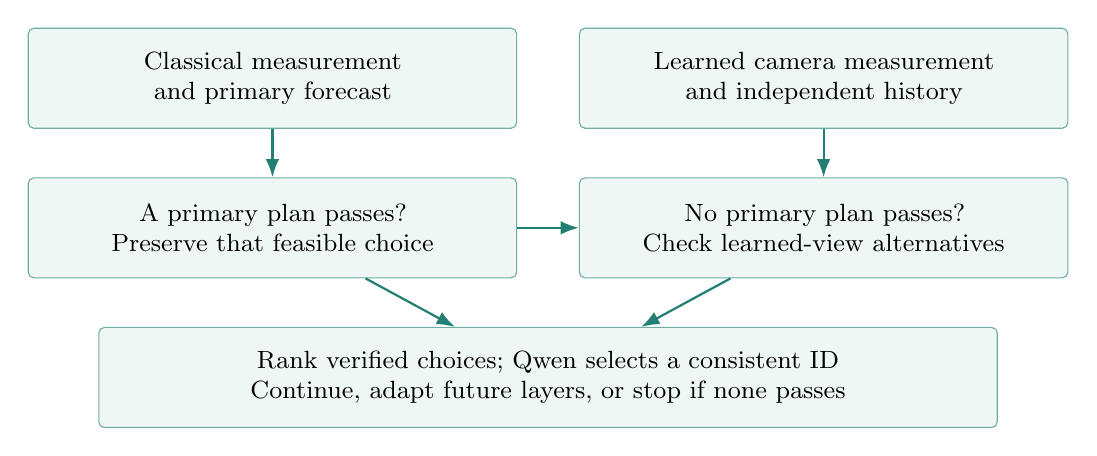
\begin{tikzpicture}[>=Latex,
  flowbox/.style={draw=teal!65,rounded corners=2pt,fill=pale,align=center,font=\small,
               text width=2.35in,minimum height=.50in},
  arr/.style={->,thick,color=teal}]
\node[flowbox] (a) at (0,0) {Classical measurement\\and primary forecast};
\node[flowbox] (b) at (7,0) {Learned camera measurement\\and independent history};
\node[flowbox] (c) at (0,-1.9) {A primary plan passes?\\Preserve that feasible choice};
\node[flowbox] (d) at (7,-1.9) {No primary plan passes?\\Check learned-view alternatives};
\node[flowbox,text width=4.4in] (e) at (3.5,-3.8) {Rank verified choices; Qwen selects a consistent ID\\Continue, adapt future layers, or stop if none passes};
\draw[arr] (a)--(c);
\draw[arr] (b)--(d);
\draw[arr] (c)--(d);
\draw[arr] (c)--(e);
\draw[arr] (d)--(e);
\end{tikzpicture}
\end{center}
The learned temporal forecast still handles specified fits using its matching
classical camera input. The camera fallback applies to parts without such fits.
This diagram describes the revision under test, not an accepted replacement.

The Qwen failure was separate: on a bracket, it described the best-ranked plan
but returned ID 1 for a different plan. IDs now match the displayed rank order.
Two actual request replays selected the intended clearance plan after this fix.
Replays verify the interface change; they are not completed-print evidence.

\subsection*{What did not improve, and the next test}
A larger camera network trained with rotations and reflections worsened boundary
validation error from 0.0792 to 0.0887 mm, so it is retained as a failed attempt.
The fallback uses the earlier checkpoint. An equivariant calibration model also
lowered displacement error but still scrapped a recoverable thinning diagnostic.
Denser training captures now target brief thinning across all three camera views;
their results and a remaining limitation are described next. New seeds 2001--2004 are reserved for
a revised frozen comparison; seeds 1001--1004 are now diagnostic data. Acceptance
still requires actual learning and Qwen calls, better completion than every
earlier baseline, preserved passing cases, and no worse defective-finish count.

\clearpage
\section{Why better camera error was insufficient}

The denser training run is complete. On the same 676,800 validation patches from
48 held-out trajectories, boundary distance error fell from 0.0838 mm for the
original camera model to 0.0731 mm for the new model, about 13\%. This did not
resolve the recoverable cup-thinning diagnostic. The actual 160-layer deposit
passes the original specification, while classical and both learned measurements
report two open walls and a support violation. Lower average distance error is
therefore insufficient evidence for better print recovery.

The new diagnostic follows the original commands throughout the print and gives
each segmenter the same actual camera frames. Simulator truth is used only for
scoring. Images and measured and true geometry at layers 84--87 are retained on
the data volume. This separates perception errors from intervention effects;
it is not a successful recovery trial.

\subsection*{Predicting between camera pixels: an unsuccessful trial}
The original network predicts one signed distance per camera pixel and then
interpolates those values. If a thin wall lies between pixel centres and all
surrounding predictions are negative, interpolation cannot recover that wall.
The next experiment predicts sixteen distinct subpixel distances from each
camera patch. It can represent a 0.0625 mm output grid while using the existing
0.25 mm camera pixels. This changes the learned representation, not the physical
camera information. No rule closes gaps or reconstructs nominal walls.

Native subpixel training uses the same 144 disjoint trajectories, dense captures
across all three views, and exact signed-distance labels at each query position.
Its completed pipeline is retained in the \texttt{native-camera-v4} window of
\texttt{neural-recovery}. Native-grid error is 0.07372 mm, but the diagnostic still
reports both false wall gaps and adds three false base-hole reports. This model
is not promoted. Old checkpoints keep their existing behavior. The full source
suite passes 94 tests, with one optional module skipped. Fresh test seeds
2001--2004 remain untouched.

\subsection*{Recovery revisions still have mixed results}
The revised camera fallback and consistent Qwen IDs restore the consumed
cup-collapse and bracket-collapse cases, including an actual agent-supervised
bracket completion with two adaptations. The fallback also loses a cup-shift
success, so it is not an accepted replacement.

A separate trial kept neural forecasting but used analytical inversion to
construct corrections. It restored two consumed spacer failures but lost all
three historical spacer-shift gains. That completed, audited ablation is retained
as negative evidence.

Keeping both inverse constructions and checking plans under both forward
forecasts performs better on that small diagnostic: all seven failure cases and
two clean controls complete, preserving the three historical gains and restoring
the two regressions. The policy uses the smaller fit slack when both forecasts
pass; if no jointly passing plan exists, it retains the original neural choices.
The optional \texttt{--neural-joint-forecast} flag enables this check. Broader
historical and actual Qwen evaluation is now complete for fit parts, as reported
next. These diagnostics do not establish superiority over the analytical policy.

\clearpage
\section{Fit recovery improves on both baselines}

The revised 291-run study is complete. It covers bracket and spacer fits,
consumed failure diagnostics, historical cases and validation. Both the earlier
and revised neural policies match their actual-Qwen variants' completion counts.

\begin{center}
\begin{tabularx}{\linewidth}{@{}Yrrr@{}}
\toprule
Comparison & Contour & Earlier neural & Revised neural\\
\midrule
Historical fit failures completed & 30/50 (60\%) & 33/50 (66\%) & 33/50 (66\%)\\
Historical defective finishes & 1 & 0 & 0\\
Historical clean controls & 10/10 & 10/10 & 10/10\\
Validation fit failures completed & 10/20 (50\%) & 12/20 (60\%) & 13/20 (65\%)\\
Validation defective finishes & 1 & 0 & 0\\
Validation clean controls & 4/4 & 4/4 & 4/4\\
\bottomrule
\end{tabularx}
\end{center}
Qwen makes 40 actual historical requests and 32 validation requests. It preserves
the neural result; these runs show no additional completed print from supervision.
These fit-only results must not be substituted for the full-project 100-case
historical comparison or for a fresh frozen test.

\note{\textbf{The earlier validation regression is resolved.} The revision retains all passing
contour and earlier-neural validation cases, including the previously lost
bracket collapse. This does not establish superiority for containers or on the
reserved fresh test.}

\subsection*{The recovery check happened one layer too late}
At bracket layer index 27, the neural forecast accepts continuation. The previous
joint implementation skipped its analytical check when only this passing choice
existed. At the next observation, the already printed hole is too small to fix.
Analytical contours intervene at 27 and finish the part.

The revised optional check also assesses that apparently healthy continuation
under the analytical forecast. Failure or low fit slack opens recovery planning
before the next layer. An alternative must pass both forecasts; when both accept
continuation, a replacement also needs more than half a camera pixel of additional
central fit slack. With no jointly passing alternative, the original neural
choice remains. This is a forecast comparison, not access to simulator truth.

The 39-run \texttt{early-joint-fit-v3} diagnostic restores the bracket but fails
its gate: an unnecessary second correction makes a previously passing spacer
finish defective, with and without Qwen. Its broader rerun is skipped. The next
guard also requires an early replacement's fit bound under both forecasts to be
at least as good as the original neural continuation's bound. That revision
passes all six bracket/spacer failure diagnostics and all four clean controls
with and without Qwen, with no defective finishes and 20 actual model requests.
The three historical gains also pass, making nine selected failure cases and
four clean controls preserved, with 30 actual model requests. The broader
50-case historical fit comparison completes at 33/50 for both neural variants
versus 30/50 for contour, with zero versus one defective finish, no lost contour
successes, all ten clean controls passed and 40 actual Qwen requests. Validation
also completes with the improvement shown above. The comparison checks the actual
earlier and current source snapshots, weights and common simulation contract.
Source tests pass 136 cases, with one optional module skipped. Seeds 2001--2004
remain untouched.

\subsection*{Local supervision now uses shorter requests}
Every eligible plan still goes to Qwen. Failed or dominated plans stay in the
full audit, and an independent check verifies that no eligible choice disappears
from the request. One actual replay reduced the user payload from 6,531 to 944
characters, kept both choices and selected the same plan. It returned in 6.65
seconds, but differing server concurrency prevents a controlled latency claim.
This replay tests the interface; it is not a new successful print.

\clearpage
\section{Camera experiments remain unsuccessful}

The camera branch has not resolved the recoverable cup-thinning diagnostic.
A signed-distance model trained for the 80th percentile reaches 80.6\% boundary
point coverage, yet still reports two false wall gaps and six false base-hole
layers. Per-point coverage is not a whole-print reliability guarantee.

An expanded dataset adds 18 complete cup and mug trajectories at a previously
missing range of thinning severity. Seeds are selected from the generator's
severity range before inspecting their outcomes. Training includes every base
frame and more samples near the deformation. The neural input remains a grayscale
camera patch. The combined split has 106 training and 56 validation trajectories,
with no shared groups. The following diagnostic used the earlier contour conversion.

\begin{center}
\begin{tabularx}{\linewidth}{@{}Yrr@{}}
\toprule
Expanded-data model & Central estimate & Upper estimate\\
\midrule
Native-grid distance error (mm) & 0.07203 & 0.09465\\
Boundary-point upper coverage & 47.2\% & 77.2\%\\
False wall-gap layers in cup diagnostic & 2 & 1\\
False base-hole layers in cup diagnostic & 3 & 5\\
Passes diagnostic specification & No & No\\
\bottomrule
\end{tabularx}
\end{center}
The actual deposit passes the original specification. Both measured stacks fail;
neither new model is promoted. As declared in advance, their conditional recovery
runs are skipped, with explicit retained reasons. The first broad measurement
validation fails after 960 frames because an invalid pixel contour crashes the
polygon union. Contours are now repaired individually before union, with tests
for the crash and preservation of visible holes. This also changes some tiny
base-hole reports: a retained identical-mask example concerns background touching
the exterior diagonally. The full 36-trajectory, 2,040-frame validation completes
under the same repaired conversion for all models. These are geometric camera
statistics, not complete-print success rates; the functional checks are unchanged.

A new camera network shares one distance decoder across subpixel XY coordinates
instead of using sixteen independent output heads. It completes 80 training epochs
on the same separated data and exports verified NumPy weights. Its 0.07351 mm
validation error is slightly worse than the central model's 0.07203 mm. The
completed cup diagnostic still reports two false wall gaps and a false support
violation; its conditional recovery trial is skipped. Both models lose their
base-hole reports under the repaired conversion, so that change is not evidence
for the shared decoder. Its geometric validation also completes; the model is not promoted.

The camera-fallback diagnostic also completes at 16/24 for both neural variants,
matching contour, but with one defective finish versus zero. It remains a rejected
replacement. The broader validation without Qwen finishes at 21/40 versus
contour's 19/40, with zero versus one defective finish and all eight clean controls
passed. The original frozen comparison completes unchanged and fails acceptance.

\clearpage
\section{Camera validation and remaining failures}

Across the completed validation set, 57 of 1,176 wall frames contain a real
opening. All 864 base frames are negative for the base-problem flag. Thus the
sample estimates false base alarms, but cannot establish base-fault recall.

\begin{center}
\begin{tabularx}{\linewidth}{@{}Yrrr@{}}
\toprule
Measurement model & False wall gaps & Missed gaps & False base alarms\\
\midrule
Classical & 66 & 3 & 0\\
Original neural & 63 & 5 & 0\\
Expanded-data central & 49 & 6 & 259\\
Expanded-data upper & 39 & 7 & 270\\
Shared-query decoder & 51 & 6 & 165\\
Matched fine-only model & 48 & 5 & 55\\
Wider-context model & 51 & 6 & 134\\
\bottomrule
\end{tabularx}
\end{center}
Newer networks detect more thinning, but fewer false wall gaps come with more
missed gaps and many false base alarms. Frames from one trajectory are correlated;
these counts are not independent trials or complete-print success rates. None of
these camera replacements is accepted.

\subsection*{Cross-checking a proposed correction}
An optional camera check retains independent classical and learned measurements
of every frame. When classical continuation fails but correction is possible,
each view assesses corrections proposed by both. A jointly passing alternative
can replace a correction rejected by the other view. Without one, preserve the
original proposal. Passing classical continuation remains unchanged. These are
two interpretations of one image, not two physical cameras.

The completed candidate comparison passes 3/4 selected failures versus contour's
2/4 and ignore's 4/4, with no defective finishes and both clean controls passed.
Qwen makes 19 actual requests and matches neural-only results. The shifted cup
now completes with one correction, but the false-gap thinning case still scraps.
That lost ignore success fails acceptance. The matched previous fallback completes
2/4; the learned camera alone completes 1/4 and finishes one defective print.
All 36 planned rows are audited. The zero-call thinning shard is explicitly
\texttt{not\_reached}, not actual supervision; its original audit failure is retained.

\subsection*{More image context, with a matched ablation}
The wider camera adds a stride-four 9-by-9 image patch to the fine patch. Both
inputs come from the existing image; renderer and functional checks are unchanged.

The experiment uses all 66 training and 36 validation container trajectories,
with 86,400 patches and whole-trajectory separation. A fine-only model trains on
the identical rows, targets, seed and optimizer schedule. Both complete 160
epochs with verified NumPy export. On the same 30,600 validation patches, boundary
error is 0.06493 mm for the fine-only model and 0.04817 mm with context. Yet the
completed cup diagnostic still reports two false gaps and a false support failure;
its conditional recovery trial is skipped. The complete geometry check favors the
fine-only model on all three error counts above, despite its higher patch error.
A retained image shows the thin wall fragmented by the prediction: average error
hides a local failure. A shared distance decoder with the same wider inputs trains
to 0.04462 mm on the identical validation patches, yet still reports two false
gaps and adds one false base-problem layer. Its recovery and wider checks are
skipped as predeclared. Both models remain rejected; no completed-print improvement
is claimed from their lower average error.

\subsection*{Evidence and next acceptance check}
See \repo{docs/validation/neural}{the validation evidence} and
\repo{docs/neural-recovery-plan.md}{the development protocol}. Full snapshots,
weights and Qwen logs stay on the data volume. Cross-version checks pin code,
options and models while holding simulation and functional checks fixed.
Acceptance requires all parts and failures, the strongest prior neural and
analytical baselines, preserved passing cases and no extra defects on a fresh test.

\clearpage
\section{Broader fit regression and the latest camera trial}

The completed \texttt{fit-consumed-grid-v5} study covers every fit case in the
consumed seed grid: three printer profiles, bracket and spacer, five failure
kinds and four seeds, plus clean controls. All 576 runs and their audits finish.
These are development cases; fresh seeds 2001--2004 remain untouched.

\begin{center}
\begin{tabularx}{\linewidth}{@{}Yrrr@{}}
\toprule
Policy & Successful failures & Defective finishes & Clean passes\\
\midrule
Contour & 71/120 & 3 & 24/24\\
Analytical preventive & 76/120 & 0 & 24/24\\
Revised neural & 78/120 & 0 & 24/24\\
Revised neural with Qwen & 78/120 & 0 & 24/24\\
\bottomrule
\end{tabularx}
\end{center}
Qwen makes 158 actual requests and preserves the neural-only result. This
demonstrates exercised supervision, not additional successful prints caused by it.

\note{\textbf{This candidate still fails acceptance.} Against analytical preventive
recovery it gains three cases but loses one: CoreXY bracket shift, seed 1001.
A higher total alone does not satisfy the requirement to preserve baseline successes.}

\subsection*{Why the remaining fit case is lost}
At layer index 26, the neural forecast still accepts continuation. The analytical
forecast predicts a failed hole fit and has a correction that completes the
physical simulation. The neural policy waits and scraps at index 27, when the
already printed hole cannot be repaired by changing future commands.

An observational replay records the otherwise discarded candidate assessments.
The analytical correction passes both central forecasts, but its neural fit bound
under the uncertainty scenarios is $-0.150$ mm, below the passing continuation's
$-0.014$ mm. The guard therefore rejects it. These are geometric scenario bounds,
not probabilities. Simple mixtures of the two inverse corrections also fail
that guard in a candidate-only diagnostic.

The new optional \texttt{--neural-hole-envelope} proposal retains both models'
compensated hole openings in future commands, keeping the neural proposal's
exterior. It changes neither measurements nor the printed prefix. Both forward
checks and the original robustness guard still apply. This raises the limiting
diagnostic bound to $+0.047$ mm. In the actual simulation, the previously lost
bracket now completes with one adaptation for both neural variants; Qwen makes
two validated requests. The 51-run gate passes all 11 selected failures and six
clean controls for both neural variants, with 38 actual Qwen requests and no
defective finishes. The broader comparison completes at 79/120 for both neural
variants versus analytical preventive recovery's 76/120 and the previous neural
policy's 78/120. All prior successes are preserved, with zero defective finishes
and all 24 clean controls passed; Qwen makes 161 actual requests. Historical and
validation fit checks tie the previous best at 33/50 and 13/20, preserving all
passing cases and clean controls with no defects. The option remains off by
default; fresh acceptance is required.

\subsection*{Explicit material classification did not fix the camera}
The \texttt{occupancy-camera-v10} trial adds a fixed classification term to the
distance objective, using the same fine-only inputs, data, seed and 160-epoch
schedule. Its zero-weight control reproduces every array of the earlier model
exactly. Both trained models export successfully to NumPy inference.

Near-boundary sign accuracy worsens from 82.09\% to 81.35\%, and boundary error
rises from 0.06493 to 0.06604 mm. On the full 160-layer cup diagnostic, both false
wall gaps remain and the false support violation grows from 15 to 23 mm$^2$.
The predeclared condition skips recovery and wider geometry trials. This network
is retained as a failed experiment and is not promoted into the recovery loop.

Rotating and reflecting image patches and their continuous queries also fails.
The unaugmented control exactly reproduces the earlier shared-query checkpoint.
Augmentation worsens boundary error from 0.04462 to 0.05504 mm, retains both false
gaps and raises false base-problem layers from one to eight. This checkpoint is
rejected; follow-up recovery and wider validation are skipped. Reserved test
seeds remain untouched.

\clearpage
\section{Learning from two observed camera frames}

The camera studies still lose thin walls that are physically present. A new
coverage analysis finds missed near-boundary material in training examples as
well as validation. The \texttt{temporal-camera-v12} experiment therefore tests
an additional observed image: the immediately preceding layer. This may help
distinguish faint current material from older layers visible underneath. It is
an experiment, not an accepted improvement.

\begin{center}
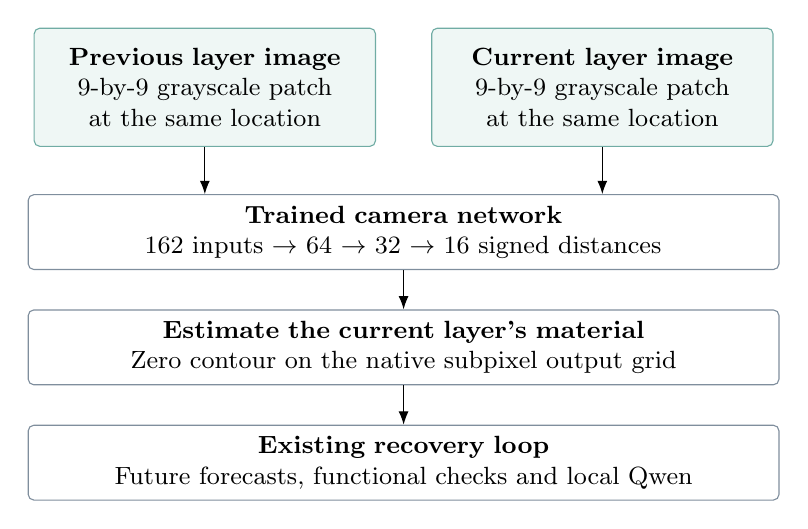
\begin{tikzpicture}[>=Latex,
 frame/.style={draw=teal!65,fill=pale,rounded corners=2pt,text width=4.1cm,align=center,minimum height=1.5cm,font=\small},
 stage/.style={draw=navy!55,rounded corners=2pt,text width=9.3cm,align=center,minimum height=0.95cm,font=\small}]
\node[frame] (previous) {\textbf{Previous layer image}\\9-by-9 grayscale patch\\at the same location};
\node[frame,right=0.7cm of previous] (current) {\textbf{Current layer image}\\9-by-9 grayscale patch\\at the same location};
\node[stage,below=0.6cm of previous.south east,xshift=0.35cm,anchor=north] (network) {\textbf{Trained camera network}\\162 inputs $\rightarrow$ 64 $\rightarrow$ 32 $\rightarrow$ 16 signed distances};
\node[stage,below=0.5cm of network] (geometry) {\textbf{Estimate the current layer's material}\\Zero contour on the native subpixel output grid};
\node[stage,below=0.5cm of geometry] (loop) {\textbf{Existing recovery loop}\\Future forecasts, functional checks and local Qwen};
\draw[->] (previous.south)--(network.north -| previous.south);
\draw[->] (current.south)--(network.north -| current.south);
\draw[->] (network)--(geometry);
\draw[->] (geometry)--(loop);
\end{tikzpicture}
\end{center}

This network estimates only the current layer. The separate learned deposition
model predicts future layers. No nominal geometry, failure identity, simulator
truth or future image enters the camera network. At the first layer, both input
slots use the current image. Later calls retain the preceding observation;
they do not acquire a second current-layer image or alter the measured prefix.
Legacy checkpoints keep their one-image behavior.

\subsection*{A matched control and explicit history handling}
The study reuses all 66 training and 36 validation trajectories. A three-trajectory
check covers 165 current frames and 156 predecessor renders across all three
views: every current input and target exactly matches the retained dataset.
An independent renderer supplies the prior image with independent camera noise,
preserving the current-image sequence. These are re-rendered camera samples,
not new physical printing trials.

The full 86,400-patch build preserves all current inputs, targets, groups and
splits exactly. A model trained on only current-image columns exactly reproduces
the earlier fine-only checkpoint. Both variants completed 160 epochs. Offline geometry
validation supplies the immediate predecessor for every selected frame; it never
uses the last selected frame when intervening layers were skipped.

Boundary error improves from 0.06493 to 0.06174 mm and near-boundary sign accuracy
from 82.09\% to 82.64\%. However, the full-stack cup diagnostic retains two false
wall gaps and adds one false hard-thin layer, despite eliminating the false
support violation. The checkpoint is rejected; conditional recovery and wider
geometry trials are skipped. All-part, fresh-test superiority remains unproven.

\clearpage
\section{Training for connected camera geometry}

A diagnostic on the retained layer-85 image finds that the central air region
already connects to the image exterior in both the fine-only and two-image
networks' native pixel masks. This occurs under both four- and eight-neighbor
background connectivity, before mask-to-contour conversion. The source images,
model hashes and diagnostic procedure are retained. This is one consumed frame,
not a fresh recovery benchmark. True geometry sampled on the identical native
grid retains a closed wall under both connectivity definitions, enclosing
1704.50 mm$^2$. The output grid can represent the missing connection.

The \texttt{dense-topology-camera-v13} experiment tests spatial supervision.
It follows the soft-clDice formulation of Shit et al., CVPR 2021
(\url{https://arxiv.org/abs/2003.07311}), which compares predicted material and
reference centre lines. Here it is an experimental training objective, with no
claim that minimizing it guarantees a valid printed part.

\subsection*{The matched experiment}
Both models retain the two-image camera architecture and train on the same 102
retained trajectories. Each selected image contributes one 24-by-24 input tile,
including the existing 9-by-9 convolution's border. The outputs are a contiguous
64-by-64 signed-distance grid at quarter-pixel spacing. Labels are clipped to
$[-1,1]$ mm and stored in half precision. Entire trajectories remain separated
between training and validation.

The control uses the existing weighted distance objective. The candidate adds a
fixed 0.1 weight on equally weighted soft-Dice and soft-clDice losses, with 20
soft-skeleton iterations and a 0.1 mm distance-to-logit scale. Homogeneous tiles
omit the clDice term. Both models use the same initialization, sample order,
40-epoch schedule and per-objective validation selection rule. Truth supplies
training labels and sampling locations only. Runtime receives observed images;
there is no morphology-based repair or change to physical or functional limits.

\subsection*{Verification and acceptance}
The dense convolution exports to the existing NumPy/OpenCV runtime. Focused tests
verify native-coordinate alignment, image-border handling and numerical parity
with full-frame inference. The loss penalizes both a removed wall segment and an
invented bridge. All three focused checks pass in the Torch environment; the
project suite passes 139 tests with two optional modules skipped.

Both 40-epoch runs complete with verified exports. The control trains in 46
seconds and the connectivity model in 746 seconds. Boundary error is 0.07839
versus 0.07911 mm; near-boundary sign accuracy is 78.73\% versus 77.73\%.

\note{\textbf{The full-print diagnostic still fails.} Both models invent open
walls at layers 85 and 86 of the simulated 160-layer cup whose true geometry
passes the specification. The distance
control also introduces a false base alarm and false support violation. The
connectivity model removes those extra alarms, but retains both false wall gaps.}

The checkpoint is rejected. Its conditional recovery and wider geometry trials
are skipped under the predeclared gate. No new recovery success is claimed;
reserved seeds 2001--2004 remain untouched. Logs, source and failed results are
retained on the data volume. The following sampling audit checks whether the
training tiles adequately represent the very thin surviving material.

\clearpage
\section{Rare thin material and commanded geometry}

An exact replay verifies every target in the 5,760-tile dense dataset. Only 39 of
3,720 training tiles contain the selected very thin surviving material, totalling
1,648 positive points. Validation has 26 such tiles and 1,147 positive points.
The diagnostic identifies material lost by a discrete 0.15 mm-radius opening on
the existing native grid, excludes nominal thin pixels, and uses a halo to avoid
crop-edge effects. This is an analysis of training exposure; it does not change
runtime geometry or functional checks.

\subsection*{Rebalancing helps recall but fails the print diagnostic}
The \texttt{balanced-camera-v14} trial places half the training sampling mass on
the 39 identified tiles and half on the remaining training tiles. It samples with
replacement, retaining the same number of samples per epoch, distance loss and
40-epoch schedule. Validation never supplies training samples or sampling mass.
The unweighted control reproduces every earlier dense-distance checkpoint array
and its file hash. Both exports pass numerical checks.

\begin{center}
\begin{tabular}{@{}lrr@{}}
\toprule
Measurement & Distance control & Balanced training \\
\midrule
Thin-material recall, training & 21.54\% & 56.98\% \\
Thin-material recall, validation & 6.02\% & 21.62\% \\
Validation boundary error & 0.07839 mm & 0.08212 mm \\
False wall gaps in the cup & 2 & 1 \\
False base alarms in the cup & 1 & 8 \\
\bottomrule
\end{tabular}
\end{center}

The layer-86 false gap disappears, but layer 85 remains open in the estimate and
one false hard-thin layer appears. The model fails its predeclared gate. Recovery
and wider geometry trials are skipped; no successful recovery is credited.

\subsection*{Commanded geometry removes gaps but does not yet pass}
The \texttt{command-camera-v15} experiment appends a binary commanded-layer
mask to the current and preceding observed image tiles. The mask comes from the
captured command, not the actual deposit. The builder verifies every old target
and retains all image inputs, targets, groups and splits bitwise. Training truth
still serves only labels and sampling checks.

The image-only balanced control reproduces v14 exactly. Both models use the same
sample weights, loss and training schedule; different input dimensions mean
identical parameter initialization is not claimed. Both exports pass, and boundary
error falls from 0.08212 to 0.07876 mm. The full-stack cup diagnostic removes both
false wall gaps, but retains two false base alarms and one false hard-thin layer.
It still fails; recovery and wider geometry checks are skipped. This is a camera
diagnostic improvement, not an accepted recovery result.

The best validation score occurs at epoch 40. A predeclared 160-epoch extension
uses identical data, sampling and loss. Training finishes, but the
export check fails: the largest float32 Torch/NumPy difference is 0.000010848 mm,
just above the 0.000010 mm tolerance. A float64 reference attributes this to
accumulation precision; one of 8,355,840 output signs differs. The failed run is
retained. A replay verifies all 160 training records and learned weight arrays
are identical, with explicit float64 inference. Export error falls to
0.000006810 mm, passing the unchanged tolerance. Boundary error improves to
0.06862 mm, but the full cup diagnostic reintroduces one false wall gap and retains
two false base alarms and one false hard-thin layer. It is also rejected.

A separate audit of all 2,040 validation tiles finds missing-material point
recall of 91.70\% for 40 epochs and 92.18\% for 160 epochs. These are points where
material is truly absent inside the commanded shape, not recovery successes.
The audit does not replace whole-print geometry validation. Conditional recovery
and wider geometry trials are skipped after the failed gate.

All long jobs run in tmux session \texttt{neural-recovery}, with retained logs and
exit status. The latest 18 focused model checks pass, including both inference
precisions, commanded-mask export parity and rejection of malformed masks.

\clearpage
\section{Testing camera errors in the recovery loop}

\subsection*{Spatial training and offset diagnostics}
The \texttt{gradient-camera-v18} trial adds a loss matching adjacent predicted
signed-distance differences to the labeled differences. It uses the same tiles,
initialization, sampling, split and 40-epoch schedule as the commanded-mask
model. The zero-weight control reproduces that checkpoint exactly. All numerical
exports pass, but neither candidate passes the unchanged 160-layer cup check.

\begin{center}
\begin{tabular}{@{}lrrrr@{}}
\toprule
Gradient weight & Boundary error & False gaps & False bases & Hard-thin alarms \\
\midrule
0 (control) & 0.07876 mm & 0 & 2 & 1 \\
0.1 & 0.08678 mm & 2 & 1 & 1 \\
0.3 & 0.08631 mm & 2 & 0 & 0 \\
\bottomrule
\end{tabular}
\end{center}

Both candidates are rejected, with conditional follow-ups skipped. A separate
audit checks whether a uniform signed-distance offset is justified. Within
0.15 mm of the true boundary, mean target minus prediction is $-0.01629$ mm in
training and $-0.01377$ mm in validation; the wall-only means are $-0.00715$ and
$-0.00299$ mm. A blanket positive offset to thicken the estimate opposes these
average residuals. None is applied; average bias does not explain every rare
thin-wall error.

The \texttt{command-base-topology-v20} diagnostic examines the raw mask on the
first five cup frames. False holes at layers 0 and 4 are disconnected from the
exterior under both four- and eight-neighbor background connectivity. Each
converted hole is 0.000335 mm$^2$, compared with 0.003906 mm$^2$ per native pixel.
The layer-0 hole lies in actual material; the layer-4 pockets are enclosed by an
erroneous predicted bulge. These are model errors before contour conversion,
distinct from the earlier diagonal-connectivity issue. No runtime hole filling
or relaxation of the specification is introduced.

\subsection*{A specification-based camera alternative}
The \texttt{base-wall-recovery-v21} study tests completed recovery directly.
An optional alternative history uses classical geometry on the specification's
solid-base layers and learned geometry on walls. Both models process every
actual image, preserving the network's preceding-image input. The primary
history remains classical, and neither history rewrites earlier observations.
Selection uses the original part specification, not fault identity or truth.
Qwen still chooses only eligible plans under the existing checks.

The protocol compares neural-only and actual Qwen against a same-checkpoint
ablation without the base split and all six prior methods: four fault cases and
two clean controls per method, 54 rows in total. Old raw results retain their
own source, model and supervisor provenance. A broader container run is
conditional on passing all six gate cases. All 54 rows are complete and audited.
Both new variants score 2/4 fault cases, versus 3/4 for the previous joint-camera
policy and 4/4 for ignore, with zero defective finishes and both clean controls
passed. Qwen makes 12 actual requests and ties neural-only. The same-checkpoint
ablation without the split also scores 2/4. The thinning case scraps at layer 86;
the shifted cup loses a previous success after one adaptation. The hybrid is
rejected and the broader follow-up is skipped.

The next full-grid trial retains analytical container measurements and forecasts,
with the improved learned forecast for specification-defined fit parts. It completes
576 new cases with and without Qwen, against the original 4,320 baseline rows.
One frozen policy is rerun on every part; old fit and container counts are not
added together as a new result. The complete development comparison reaches
136/240, detailed on page 23. Historical regression and a new frozen test remain
required; fresh seeds 2001--2004 are untouched.

The camera-change checkpoint passes 141 tests with two optional modules skipped. Focused
checks verify the training loss, both camera histories and full/partial base
frame accounting. Logs, failed experiments and source snapshots are retained.

\clearpage
\section{Retaining actual rescues in the full policy}

\subsection*{A successful print is not always a recovery}
Many fault-injected prints still meet their specification without a correction.
The comparison therefore separates functional completions from actual rescues:
a rescue finishes successfully when the matched \code{ignore} run fails. A
retrospective accounting of the original 4,320 rows gives the following results
on 240 fault cases per policy.

\begin{center}
\begin{tabular}{@{}lrrrr@{}}
\toprule
Original policy & Completions & Rescues & Lost ignore passes & Defective finishes \\
\midrule
Analytical preventive & 133 & 15 & 10 & 3 \\
Combined neural & 129 & 15 & 14 & 4 \\
Combined neural + Qwen & 126 & 12 & 14 & 5 \\
\bottomrule
\end{tabular}
\end{center}

Every completed print with zero adaptations matches its ignore counterfactual.
This supports attributing the observed rescues to changed commands in this
simulator. It does not prove real-printer causality or generalization. The new
full runs must improve completed outcomes while retaining prior successes and
controlling defective finishes; model calls alone earn no recovery credit.

\subsection*{Preserve earlier container rescues}
The \texttt{joint-historical-gate-v23} study checks the complete improved fit
policy with analytical containers against the same policy retaining the earlier
trained camera as an independent second opinion. It uses the existing joint
forecast checks and the original camera checkpoint, not a rejected replacement.
Both variants run with and without actual Qwen on two known bedslinger cases:
cup under-extrusion and mug shift, seed 10, plus two clean controls. Contour and
ignore are rerun under the same frozen source as paired controls.

All 24 rows finish and pass audit. Analytical containers and contour complete
0/2 fault cases; ignore finishes both defective. Both joint-camera variants
complete 2/2, with zero defective finishes and both clean controls passed. The
cup uses one adaptation and the mug three. Qwen makes 11 actual requests and
matches neural-only outcomes. These are preserved historical rescues, not new
untouched successes or proof of the best overall policy.

The gate passes. Its complete 576-row follow-up reaches 141/240 successes but
five defective finishes, detailed on page 25. Each run uses one frozen policy on
every part, with separate raw results and matched neural-only/Qwen outcomes.
Historical regression and a new untouched comparison remain required.

\subsection*{Verify earlier workers without rewriting their records}
The original Qwen workers recorded an asset-only attestation and a richer server
attestation. The comparison now pins each exact input manifest and retains both
records. A separately pinned runtime check verifies matching model assets and
inference command settings; only server addresses and JSON whitespace are
normalized. Changed models, settings, evidence or unused shard pins fail checks.
All 23 focused provenance tests pass. Replaying the full original comparison
reproduces all 15 policies' outcome and inference counts, paired gains and losses,
and defective-finish differences across the unchanged 4,320 rows.

The new studies run in tmux session \texttt{neural-recovery}. Complete audits,
source snapshots, checkpoint hashes and actual model requests remain available.
Fresh seeds 2001--2004 remain untouched, and the overall objective is unmet.

\clearpage
\section{A modest gain on the complete development grid}

\subsection*{Complete comparisons, with the remaining losses visible}
The \texttt{fit-analytical-containers-v22} run finishes and passes audit: 576 new
rows plus all 4,320 original rows, covering 17 separate configurations. One
frozen policy uses classical camera measurements throughout, learned forecasts
and shared-hole recovery proposals for specified fits, and analytical container
forecasts. All three profiles, four parts, five faults and clean controls are
included on consumed seeds 1001--1004.

\begin{center}
\begin{tabular}{@{}lrrrr@{}}
\toprule
Policy & Completions & Rescues & Defective & Clean \\
\midrule
Earlier analytical preventive & 133/240 & 15 & 3 & 48/48 \\
Matched current analytical & 133/240 & 15 & 1 & 48/48 \\
Latest neural & 136/240 & 18 & 1 & 48/48 \\
Latest neural + Qwen & 136/240 & 18 & 1 & 48/48 \\
\bottomrule
\end{tabular}
\end{center}

Every earlier analytical success is retained. The three gains are spacer shifts
at seed 1002, one per profile. The latest policy completes 109 fault cases without
adaptation and 27 after adaptation; 18 are rescues that the matched ignore policy
fails. It still loses ten ignore successes, as does the earlier analytical policy.
It also loses successes of other earlier policies and the two historical camera
rescues discussed on the preceding page. Its one defective finish is bedslinger
mug under-extrusion at seed 1004. Qwen makes 499 actual requests and adds no
completions over neural-only. The neural forecast makes 236,556 calls on fault
cases and 2,064 on clean controls.

\subsection*{Separate learning from accompanying measurement changes}
The earlier analytical baseline used an older contour-conversion implementation.
\texttt{matched-analytical-v26} completes all 288 analytical-control cases with
the exact current source and classical camera used above. It makes no neural or
agent calls and retains a separate comparison label. The combined 5,184-row
comparison confirms 136/240 versus 133/240, with every analytical success retained
and one defective finish each. The three gains remain the spacer shifts. Thus
the learned policy adds three rescues; the earlier reduction from three defects
to one also occurs without learning. The difference includes forecasting and
associated proposals, not a pure forecast-only ablation. Fresh-test superiority
remains unproven.

The initial neural-only auditor refused a control with no model. A tested
\texttt{--analytical-only} mode now requires analytical methods, no model assets
and zero learned/agent calls. All 38 audit/provenance checks pass. Re-auditing
the 576 neural rows preserves the earlier results, including 499 agent calls.
Only audit/comparison resumes; failed logs and all original raw runs are retained.

\subsection*{Two additional camera ideas fail their gates}
Fixed equal averaging of the short- and long-trained signed-distance outputs
retains one false wall gap, two false base layers and one false hard-thin layer
on the complete known cup trajectory. Both member controls reproduce exactly.
Classical bases remove only the base alarms; averaging is rejected.

Tripling the training cost of underpredicted signed distance also fails. Its
unit-weight control exactly reproduces the earlier checkpoint, and both exports
pass. Validation boundary error worsens from 0.07876 to 0.09269 mm and sign
accuracy from 78.11\% to 74.20\%. The candidate retains one false gap, two false
base layers and two false hard-thin layers. The wider follow-up is skipped and
no recovery credit is claimed. This asymmetric loss is not a calibrated
confidence bound. Eight focused Torch tests pass; the default loss is unchanged.

Full raw results, pinned sources and rejected models remain on the data volume;
compact evidence is retained in the repository. The report does not claim a
physical-printer result or an accepted overall winner.

\clearpage
\section{What the false thickness alarm measures}

\subsection*{Invented material can make a measured wall look too thin}
The minimum-wall check uses the fraction of material removed by a morphological
opening, relative to the nominal layer. It can therefore reject a prediction
with spurious narrow protrusions even when the real wall passes. The retained
\texttt{thin-attribution-v27} analysis partitions the short-trained camera's
thin region on the known cup's layer 86:

\begin{center}
\begin{tabular}{@{}lr@{}}
\toprule
Predicted thin material lies & Area (mm$^2$) \\
\midrule
Inside actually thin material & 6.1633 \\
Inside actually thick material & 0.2431 \\
Outside the actual deposited material & 2.0401 \\
\bottomrule
\end{tabular}
\end{center}

The partition reproduces the metric after accounting for the opening's small
exterior area. Predicted thin excess is 0.030745, above the unchanged 0.03 limit;
actual excess is 0.024405. Removing contour simplification worsens it to 0.037241.
Truth explains this error retrospectively; it is never a runtime input.

\subsection*{Train a small spatial output layer with the camera held fixed}
The \texttt{native-refinement-v28} experiment keeps every existing camera weight
fixed and learns a 3-by-3 convolution plus bias on the native distance logits,
before the final tanh: ten new parameters, initialized to identity. Adjacent
output positions can influence one another across the original pixel blocks.
The network still receives only observed images and the commanded layer mask.

Training uses the original distance loss, balanced training-only sampling and
40 epochs. Valid convolutions score the common 62-by-62 tile interior, excluding
artificial crop-edge padding. Base and refinement use the same dataset and the
same disjoint 66 training and 36 validation groups. Validation loss selects the
weights; the known cup's outcome does not choose an epoch or kernel.

\begin{center}
\begin{tabular}{@{}lrr@{}}
\toprule
Matched tile-interior metric & Identity control & Learned refinement \\
\midrule
Boundary MAE (mm) & 0.078446 & 0.072209 \\
Near-boundary sign accuracy & 78.16\% & 80.50\% \\
\bottomrule
\end{tabular}
\end{center}

Training takes 21.2 seconds. Base weights remain identical. Export disagreement
is 0.000006527 mm, below the unchanged 0.000010 tolerance. Full-image inference
agrees across block boundaries; identity preserves the old field exactly.
All 24 focused checks pass; the repository suite passes 147 tests with three
optional modules skipped.

The complete 160-frame cup diagnostic passes for both the raw refined camera and
its classical-base alternative: no false gap, base, thickness or overhang
failures. Original and identity controls exactly reproduce the earlier two false
base layers and one false hard-thin layer. Every model observes all 160 frames.
The complete 2,040-frame validation rejects the model: it misses ten of 57 real
gap frames, versus five for the original camera. False gap alarms fall from 63
to 35. Severe-thinning misses improve from 40 to nine, but false thinning alarms
rise from zero to 16. False base alarms fall from the commanded control's 452
to five; no true base failures occur in this validation set. These improvements
do not waive the missed-gap gate. Passing a known diagnostic earns no recovery
credit, and the learned output layer is not a calibrated confidence bound.

The conditional \texttt{refined-recovery-gate-v29} comparison requires both main
variants to pass six fault cases and four clean controls without defective
finishes. It retains earlier configurations and a camera ablation. The failed
geometry gate skips this run: zero recovery rows are executed or credited.
Original orchestration failures and the successful audit-only repair are retained.

The follow-up \texttt{gap-sensitive-refinement-v30} doubles the training cost of
invented material, retaining data, groups, initialization and epochs. Its control
reproduces v28 exactly. Boundary error is 0.074073 mm versus the control's 0.072209;
both exports pass. However, two false wall gaps return in the full cup diagnostic,
with or without classical bases. The model is rejected before broader validation
or recovery. All 25 focused tests pass; camera improvement remains unproven.

\clearpage
\section{More completions, but an unacceptable defect trade-off}

\subsection*{The complete joint-camera comparison}
The \texttt{joint-historical-gate-v23} follow-up completes all 576 rows. Adding
the same-code analytical control in \texttt{joint-matched-comparison-v31} produces
5,760 audited rows across 20 configurations. All 19 earlier summaries remain
identical; no simulation is rerun or pooled under a changed policy label.

\begin{center}
\begin{tabular}{@{}lrrrr@{}}
\toprule
Policy & Successes & Rescues & Defective & Clean \\
\midrule
Matched analytical & 133/240 & 15 & 1 & 48/48 \\
Prior neural + Qwen & 136/240 & 18 & 1 & 48/48 \\
Joint-camera neural & 141/240 & 18 & 5 & 48/48 \\
Joint-camera neural + Qwen & 141/240 & 18 & 5 & 48/48 \\
\bottomrule
\end{tabular}
\end{center}

Every success from the active recovery baselines is retained. Five ignore
successes remain lost, down from ten. Qwen makes 527 actual requests and adds
no completions over neural-only. The five gains over the prior candidate are
cartesian cup collapse/1003 and shift/1002, corexy mug collapse/1001 and warp/1001,
and bedslinger mug warp/1001. Four finish without adaptation; one uses a
correction. These restore usable prints; genuine rescues remain 18.

Four additional defective finishes follow corrections supported only by the
learned camera when no classical plan passes: mug under-extrusion/1002 on all
three profiles and corexy mug under-extrusion/1004. All those alternatives have
robust margin $-1$: their existing uncertainty envelope fails. The prior
bedslinger mug under-extrusion/1004 defect remains. The five remaining lost
ignore successes are all scrapped before adaptation. Recorded reasons guide
the next experiment; they are not causal proof of a simulation failure.

\subsection*{Test a guard on unsupported corrections}
The opt-in \texttt{--boundary-robust-fallback} requires a finite existing robust
margin of at least zero for a learned-camera correction when no classical plan
passes. Rejected alternatives remain in the audit and cannot be eligible Qwen
choices. Passing continuations and jointly checked corrections keep their
existing behavior. Both historical rescues and successful container corrections
in the full grid used jointly checked plans, motivating this distinction.
The geometry specification and uncertainty calculation do not change; the
guard is not a calibrated probability.

The \texttt{robust-fallback-v32} run tests 42 rows: five new gains, four extra
defects, the prior defect, two historical rescues, three learned fit gains and
six clean controls, with and without Qwen. Both methods must retain all ten
reference fault successes and six clean controls, introduce no new defective
case and finish at most the one previously defective case. Actual neural,
camera and agent calls are required. All 42 rows complete and pass audit. Each
variant retains ten fault successes and six clean controls, stops the four extra
defective prints without adaptation, and retains the one existing defect.
Each makes 104,468 neural and 2,280 boundary queries; Qwen makes 60 actual calls
and ties neural-only. This passes the targeted gate, not final acceptance.

All 159 repository tests pass, with three optional modules skipped. They check
negative/nonfinite and zero margins, default behavior, preserved continuations
and joint plans, and audit rejection of missing or bypassed guards. Re-auditing
the completed 576-row comparison preserves every prior field except the auditor
digest, including all 527 Qwen calls. Full historical regression and untouched
seeds 2001--2004 remain outstanding. No physical-printer reliability is claimed.

The conditional \texttt{robust-full-v33} run starts after all 42 targeted rows
pass. It evaluates 576 rows with twelve workers and compares all 22
configurations across 6,336 rows. The unchanged models and policy options match
the targeted run exactly. The queued \texttt{robust-historical-v34} follow-up
requires a best full-grid completion count, no higher defects, all clean controls
and retained active-recovery successes. It then tests all 100 historical faults
and 20 clean cases against eleven earlier full-domain configurations, with a
separate fit-only comparison retaining six earlier configurations. Both jobs
check storage before execution. Remaining ignore losses stay visible; these
conditional stages do not establish fresh-test superiority.

\clearpage
\section{A nonlinear camera refinement experiment}

The linear spatial head removes false alarms in a known cup print but misses
more real gaps in broader validation. The \texttt{nonlinear-refinement-v35}
experiment tests whether a local nonlinear correction can distinguish those
patterns. It freezes the same commanded temporal camera and learns 89 parameters:
a $3\times3$ convolution with eight hidden channels, ReLU, a $1\times1$ output
and a residual connection before tanh. Zero output weights and bias initially
preserve the original logits exactly. The dataset, 66 training and 36 validation
groups, sampling, symmetric loss and 40-epoch schedule remain matched.

The retrained linear control reproduces the v28 checkpoint hash exactly. Both
heads start with identical validation predictions and preserve every backbone
weight. Only full tile validation loss selects the saved checkpoint.

\begin{center}
\begin{tabular}{@{}lrrr@{}}
\toprule
Refinement & Parameters & Boundary MAE (mm) & Sign accuracy \\
\midrule
Linear control & 10 & 0.072209 & 80.50\% \\
Nonlinear residual & 89 & 0.071095 & 80.39\% \\
\bottomrule
\end{tabular}
\end{center}

The candidate's maximum Torch/NumPy export difference is 0.000008285 mm, within
the unchanged 0.000010 mm tolerance. Lower tile error does not establish fewer
missed gaps or better recovery. The full 160-frame cup diagnostic passes for
both the raw learned geometry and the classical-base hybrid, with no false gaps,
base failures, thinning or overhang. Its linear control and actual truth reproduce
exactly. The same 2,040-frame geometry comparison is running. Gap false positives,
missed gaps and severe-thinning misses may not
exceed the original camera's counts. All prior control frames must reproduce
exactly. Failed gates skip recovery, and untouched seeds remain reserved.

All 159 repository tests pass, with three optional modules skipped. In the
existing Torch environment, all 22 focused camera/export tests pass, covering
full images, native block seams, both inference precisions, exact identity
behavior and invalid checkpoint rejection. Training and diagnostics run in
\texttt{neural-recovery:nonlinear-v35} with two CPU threads and an 8 MB artifact
allowance. The separate guarded-policy benchmark retains its frozen source,
original camera and unchanged model weights.

\clearpage
\section{Separating camera errors from forecast errors}

The \texttt{forecast-attribution-v36} replay diagnoses the consumed bedslinger
mug-collapse case at seed 1001. It prints all 160 layers without changing any
commands. At layer 137, both current forecasts reproduce the recorded false
handle-connection failure near z=35.2 mm. The actual print and both complete
camera histories pass the unchanged functional specification.

\begin{center}
\begin{tabular}{@{}lcc@{}}
\toprule
Offline diagnostic & Classical camera & Learned camera \\
\midrule
Observed prefix + actual future & Pass & Pass \\
Actual prefix + current forecast & Fail & Fail \\
Observed prefix + current forecast & Fail & Fail \\
Observed prefix + latest deformation held & Pass & Pass \\
\bottomrule
\end{tabular}
\end{center}

The selected false alarm comes from future extrapolation. Holding the latest
measured deformation removes it in this diagnostic, but that does not establish
a successful recovery or a generally better forecast. Actual future geometry is
used only for offline attribution; it is never an estimator input.

The opt-in \texttt{--contour-trend-shrinkage} discounts the existing observation
uncertainty from each clipped median increment's magnitude, floored at zero.
It retains the increment's direction, the complete latest deformation, measured
history and the three-layer horizon. The trained fit forecasts are unchanged.
There is no new fitted threshold or runtime fault/outcome input, and the
uncertainty is not a calibrated confidence bound.

The \texttt{trend-shrinkage-v37} test first runs the same-source default and
candidate on the mug, both with and without actual Qwen. The default must
reproduce the prior scrap and action sequence. Both candidates must finish
successfully before all 42 earlier targeted rows run. The complete gate requires
all ten prior fault successes, the new mug success, all six clean controls and
at most the same single existing defective case. Actual neural, camera and
agent calls are required; fit rows must record zero shrinkage calls. A passing
first phase produces 46 new rows overall: two controls and 44 candidate rows.
The first four rows complete and pass audit. Both default controls reproduce the
prior scrap and action sequence; both candidates finish with zero adaptations or
defective finishes. Each records 1,190 shrinkage queries. Qwen makes three actual
candidate calls and ties neural-only. This preserves an ignore-successful print;
it does not add a genuine rescue. The 42-row preservation regression is running.
Full comparisons and untouched evaluation remain required; no overall count is
inferred from this single case.

All 164 repository tests pass, with three optional modules skipped. The 21 focused
forecast/fallback tests check unchanged observations and learned fit states,
retained deformation, suppression of small increments, preserved larger trends,
the existing horizon and propagation to both camera forecasts. The experiment
runs in \texttt{neural-recovery:trend-shrinkage-v37} with at most two simulation
workers and an 8 MB artifact allowance. The ongoing full-policy and camera
validations keep their own frozen sources.

\end{document}
